\section*{Part 2}

\begin{enumerate}
 
    \item \textbf{Interference behavior}
    \begin{enumerate}

%%%%%%%%%%%%%%%%%%%%%%%%%%%%%%%%%%%%%%%%%%%
%%% QUESTION 2.1A

        \item Fill in the following table with the normalized execution time of each batch job with each source of interference. The execution time should be normalized to the job’s execution time with no interference. Round the normalized execution time to 2 decimal places. Color-code each cell in the table as follows: {\color{Green}\textbf{green}} if the normalized execution time is less than or equal to 1.3, {\color{YellowOrange}\textbf{orange}} if the normalized execution time is over 1.3 and less or equal to 2, and {\color{Red}\textbf{red}} if the normalized execution time is greater than 2. The coloring of the first three cells is given as an example of how to use the cell coloring command.   \textbf{{\color{red}Do not change the structure of the table. Only input the values inside the cells and color the cells properly.}} 

        % Fill in this table with your results and color the cells accordingly with the \cellcolor{color} command
        \begin{center}
        \begin{tabular}{ |c|c|c|c|c|c|c|c| } 
        \hline
         \textbf{Workload} & \texttt{\textbf{none}} & \texttt{\textbf{cpu}} & \texttt{\textbf{l1d}} & \texttt{\textbf{l1i}} & \texttt{\textbf{l2}} & \texttt{\textbf{llc}} & \texttt{\textbf{memBW}}  \\
         \hline\hline
        barnes         & 1.00 & \cellcolor{YellowOrange} 1.48 & \cellcolor{YellowOrange} 1.57 & \cellcolor{YellowOrange} 1.78 & \cellcolor{YellowOrange} 1.62 & \cellcolor{Red} 2.01 & \cellcolor{YellowOrange} 1.57 \\  \hline
        blackscholes         & 1.00 & \cellcolor{Green} 1.24 & \cellcolor{Green} 1.28 & \cellcolor{YellowOrange} 1.78 & \cellcolor{YellowOrange} 1.45 & \cellcolor{YellowOrange} 1.39 & \cellcolor{Green} 1.30 \\  \hline
        canneal & 1.00 & \cellcolor{Green} 1.12 & \cellcolor{Green} 1.29 & \cellcolor{Green} 1.25 & \cellcolor{Green} 1.29 & \cellcolor{YellowOrange} 1.80 & \cellcolor{YellowOrange} 1.33 \\  \hline
        freqmine & 1.00 & \cellcolor{YellowOrange} 1.93 & \cellcolor{YellowOrange} 1.32 & \cellcolor{YellowOrange} 1.96 & \cellcolor{YellowOrange} 1.32 & \cellcolor{YellowOrange} 1.74 & \cellcolor{YellowOrange} 1.61 \\  \hline
        radix & 1.00 & \cellcolor{Green} 0.96 & \cellcolor{Green} 1.09 & \cellcolor{Green} 0.99 & \cellcolor{Green} 1.10 & \cellcolor{YellowOrange} 1.41 & \cellcolor{Green} 1.02 \\  \hline
        streamcluster & 2.00 & \cellcolor{YellowOrange} 1.58 & \cellcolor{YellowOrange} 1.39 & \cellcolor{YellowOrange} 1.49 & \cellcolor{YellowOrange} 1.39 & \cellcolor{YellowOrange} 1.84 & \cellcolor{YellowOrange} 1.39 \\  \hline
        vips & 1.00 & \cellcolor{YellowOrange} 1.64 & \cellcolor{YellowOrange} 1.73 & \cellcolor{YellowOrange} 1.71 & \cellcolor{YellowOrange} 1.69 & \cellcolor{YellowOrange} 1.90 & \cellcolor{YellowOrange} 1.76 \\  \hline
        \end{tabular}
        \end{center}

%%%%%%%%%%%%%%%%%%%%%%%%%%%%%%%%%%%%%%%%%%%
%%% QUESTION 2.1B

        \item Explain what the interference profile table tells you about the resource requirements for each job. Give your reasoning behind these resource requirements based on the functionality of each job.

        \textbf{Answer:}
        \begin{itemize}
            \item \texttt{barnes:} % What does the interference table tell you about the resource requirements for this job? - Here you place your solution.
            The job is very sensitive to the last level cache (llc). Therefore, the last level cache is highly important for the execution. The interference of other resources are also significantly effecting the execution time. This shows, that the job uses most of the resources.
            
            \textit{Explanation:} % What is the resoning behind these requirements? - Here you place your solution.
            \\ The barnes benchmark implements the Barnes-Hut approximation algorithm. Because of the usage of tree-based data structures, the tree traversals in the algorithm makes it sensitive to cache-performance. The irregular memory access patterns cause more often accesses to the last level cache, which increases its sensitivity in regards to interference of the llc. This also explains the sensitivity for l1d, l2 and memBW. The effects on interference of the l1i cache can be explained by the branching and more complex control flow of the tree traversal. Additionally, the algorithm is compute intensive, therefore the interference of cpu is causing a slowdown in execution time.
            
            \item \texttt{blackscholes:} % What does the interference table tell you about the resource requirements for this job? - Here you place your solution.
            Cpu, l1d, and memBW sharing are less important to the execution of the job. The interference of these resources barely effect the execution time. The most intensely used resources is the l1i cache, as the interference caused the biggest effect on the execution time. l2 cache and llc cache are also important, seen by the medium slowdown of the jobs.
            
            \textit{Explanation:} % What is the resoning behind these requirements? - Here you place your solution.
            \\ The barnes benchmark uses the Black–Scholes equation and computes prices of financial derivatives with a large number of options. The job repeatedly evaluates the same equation, therefore not depending on irregular data movement, explaining the cpu, l1d and memBW to be low. The effects on the l1i cache are due to the same instructions being repeated often in the code. This can also explain the effects on l2 and llc cache.

            \item \texttt{canneal:} % What does the interference table tell you about the resource requirements for this job? - Here you place your solution.
            The job is little effected by the sharing of cpu, l1d, l1i, and l2 cache, suggesting that these resources are less intensively used. memBW has a higher, but still small effect, making it a more important resource. The llc is important for the execution, as the interference had the highest effects.
            
            \textit{Explanation:} % What is the resoning behind these requirements? - Here you place your solution.
            \\ To optimize placement of components in a chip layout, canneal uses simulated annealing. The used algorithm accesses memory in an irregular way, making the algorithm memory bound. This is visible in the high latency for llc and higher latency for memBW, but the lower effects on lower level caches. That the cpu interference had little effect can also be explained by the algorithm being memory bound.

            \item \texttt{freqmine:} % What does the interference table tell you about the resource requirements for this job? - Here you place your solution.
            The runtime in interference is the highest for cpu and l1i cache, making these two the most important resources for freqmine. llc and memBW interference also show significant increase in runtime, suggesting them to also be important and well used resources. l1d and l2 cache interference has less effects, suggesting them to be of minor importance in comparison to the other resources.
            
            \textit{Explanation:} % What is the resoning behind these requirements? - Here you place your solution.
            \\ The freqmine benchmark implements the FP-growth algorithm. The algorithm includes high memory usage and irregular data access, explaining the increase in runtime when interfering with llc and memBW. The algorithm also includes complex data structure traversals and computations, explaining the sensitivity to cpu interference. The l1i cache importance shown by the measurements suggests, that the algorithm has repeating instruction patterns.

            \item \texttt{radix:} % What does the interference table tell you about the resource requirements for this job? - Here you place your solution.
            Almost all resources seem to be of minor usage in the job, not effecting the runtime of the job in any way. llc interference influenced the runtime most, suggesting that llc is an important and often used resource in the job execution. 
            
            \textit{Explanation:} % What is the resoning behind these requirements? - Here you place your solution.
            \\ The radix benchmark sorts integers using the radix sort algorithm. The low impact of interference with memBW and low level caches can be explained by the structured data access of the algorithm of large arrays. As large arrays of data are repeatedly read and accessed, the llc is important for keeping the information cached, slowing the job down when interfering with it. 

            \item \texttt{streamcluster:} % What does the interference table tell you about the resource requirements for this job? - Here you place your solution.
            The interference table shows medium slowdown for all resources. The lowest impacts have the memBW, l1d and l2 interference, suggesting that these resources not too much occupied, cpu and l1i are more important, as interfering with them leads to a greater slowdown. The biggest impact has the llc interference, which leads to the conclusion that it is of importance for the job.
            
            \textit{Explanation:} % What is the resoning behind these requirements? - Here you place your solution.
            \\ The benchmark uses a stream clustering algorithm. The algorithm has mixed workload between computation and memory and cache usage, making all resources important. The cpu slowdown is due to the heavy computation of forming the clusters. memBW interference is slowing the algorithm down, as the data for the clustering has to be fetched from memory. The repeated acces of larger amounts of data in the algorithm, makes the usage of llc more important.

            \item \texttt{vips:} % What does the interference table tell you about the resource requirements for this job? - Here you place your solution.
            The impact of the interference of the resources for the runtime of the job is very similar for all resources, but a bit higher for the llc. This suggests that all resources are similarly important for the algorithm and llc has a slightly bigger imprtance than the other ones.

            \textit{Explanation:} % What is the resoning behind these requirements? - Here you place your solution.
            \\ Vips processes large images, applying filters and transformations to them. The algorithm creates high data movement, touching large arrays of pixels and applying multiple filters to them. The reuse of parts of the data for the transformations explains the interference effects for the caches and the memBW. Additionally, the memBW interference effects how the images are fetched from memory, as they are large. As transformations are repeatedly executed, l1i cache is useful, as the instructions are already in the cache. Finally, the algorithm has to constantly transform arrays of pixels, making the job compute intensive, which is visible in the increased runtime when there is interference with the cpu.
         \end{itemize}


%%%%%%%%%%%%%%%%%%%%%%%%%%%%%%%%%%%%%%%%%%%
%%% QUESTION 2.1C
        
        \item Which jobs (if any) seem like good candidates to collocate with memcached from Part 1, without violating the SLO of 2 ms P95 latency at 40K QPS? Explain why.

        \textbf{Answer:} The results from Part 1 show, that collocating memcached with cpu and l1i cache intensive workloads has the biggest impact on runtime. All other resources show similar behavior on interference. Therefore, we should choose tasks where both, cpu and l1i cache are less heavily used. The best candidate for collocation is \texttt{radix}. It shows no effect on interference with cpu and l1i cache and very low effects for interference on l1d, l2, and llc. Therefore, it should barely effect the performance of memcached. According to the results for cpu and l1d cache, \texttt{canneal} and \texttt{balckscholes} are good candidates, too. The interference of l1i, l2, llc, and memBW showed stronger effects here. It is unknown, if and how these results could add up or not when interfering with memcached. It is likely, that both would decrease the performance of memcached more than \texttt{radix}.
        
    \end{enumerate}
    
    \item \textbf{Parallel behavior}
    \begin{enumerate}

%%%%%%%%%%%%%%%%%%%%%%%%%%%%%%%%%%%%%%%%%%%
%%% QUESTION 2.2A

        \item Plot a line graph with speedup as the y-axis (normalized time to the single thread config, $\textrm{Time}_1$ / $\textrm{Time}_n)$ vs. number of threads on the x-axis (1, 2, 4 and 8 threads - see the project description for more details). Pay attention to the readability of your graph. % it will be a part of your grade.

        \textbf{Answer:} % Here you place your solution.
        \\

        \begin{figure}[H]
            \centering
            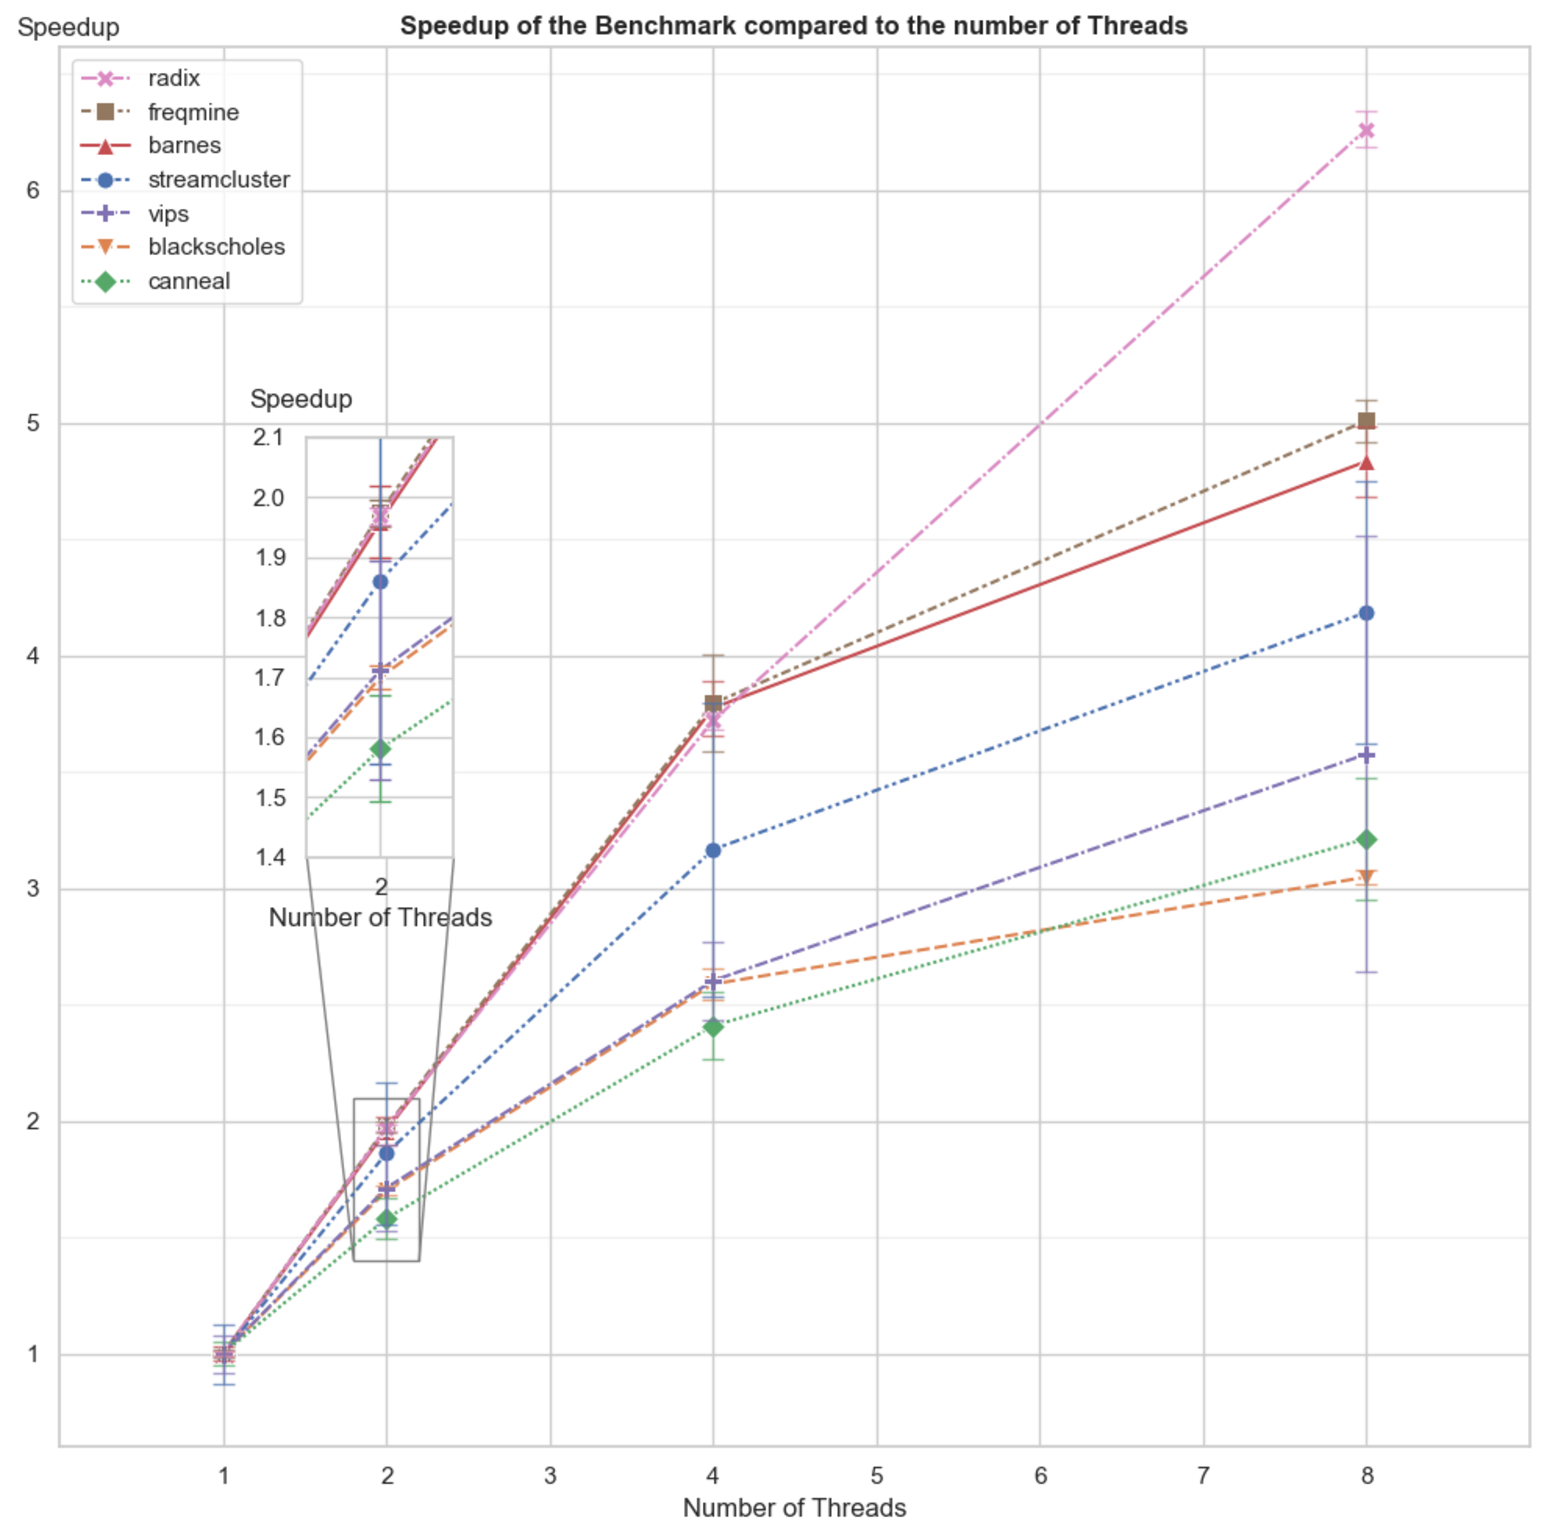
\includegraphics[width=1\linewidth]{report/figures/part2b.pdf}
            \caption{Speedup of the execution of the batch job when increasing the number of threads. For readability, inset added to the plot, showing the specific speedup for using 2 threads.}
            \label{fig:part2b}
        \end{figure}

%%%%%%%%%%%%%%%%%%%%%%%%%%%%%%%%%%%%%%%%%%%
%%% QUESTION 2.2B

        \item Briefly discuss the scalability of each job: e.g., linear/sub-linear/super-linear. Do the applications gain significant speedup with the increased number of threads? Explain what you consider to be ``significant''.

        \textbf{Answer:} In the following explanations, we consider a significant speedup to be at least $1.5 \times$ for 2 threads, $2.5 \times$ for 4 threads and $4 \times$ for 8 threads.
        \begin{itemize}
            \item \texttt{barnes:} % Discuss the scalability of this job and the significance of the speedup with a different number of threads. - Here you place your solution.
            \\ The barnes job scales sub-linearly in general, but the scale-up is linear for up to 4 threads, but not for 8 threads anymore. For all four scenarios, a significant speedup is seen, with almost $2\times$ for 2 threads, $\approx 3.75\times$ for 4 threads, and $\approx 4.75\times$ for 8 threads.
            
            \item \texttt{blackscholes:} % Discuss the scalability of this job and the significance of the speedup with a different number of threads. - Here you place your solution.
            \\ The blackscholes job has sub-linear scalability. The speedup is significant 2 threads with $\approx 1.7 \times$ and for 4 threads with $\approx 2.6 \times$. For 8 threads, there is no significant speedup, as it is at $\approx 3.05 \times$.

            \item \texttt{canneal:} % Discuss the scalability of this job and the significance of the speedup with a different number of threads. - Here you place your solution.
            \\ The canneal job has sub-linear scalability. The speedup is only significant for 2 threads with $\approx 1.6 \times$, and not significant for 4 threads, $\approx 2.4 \times$, and 8 threasds, $\approx 3.2 \times$.
            
            \item \texttt{freqmine:} % Discuss the scalability of this job and the significance of the speedup with a different number of threads. - Here you place your solution.
            \\ The freqmine job scales sub-linearly in total, but linearly for up to 4 threads. It shows a significant speedup for all situations with $\approx 2 \times$ for 2 threads, $\approx 3.75 \times$ for 4 threads, and $\approx 5 \times$ for 8 threads.

            \item \texttt{radix:} % Discuss the scalability of this job and the significance of the speedup with a different number of threads. - Here you place your solution.
            \\ The radix job has a sub-linear scalability, which is almost linear. For all number of threads it shows a significant speedup. The speedup for 2 threads is $\approx 2 \times$, for 4 threads $\approx 3.75 \times$, and for 8 threads $\approx 6.25 \times$. This job has the best scalability over all jobs.

            \item \texttt{streamcluster:} % Discuss the scalability of this job and the significance of the speedup with a different number of threads. - Here you place your solution.
            \\ The streamcluster job has sub-linear scalability, too. It shows a significant speedup for all threads, with $\approx 1.85 \times$ for 2 threads, $\approx 3.2 \times$ for 4 threads, and $\approx 4.2 \times$ for 8 threads. It shows a medium speedup with it's speedup being the median of all job's speedups.

            \item \texttt{vips:} % Discuss the scalability of this job and the significance of the speedup with a different number of threads. - Here you place your solution.
            \\ Also the vips job shows sub-linear scalability. It's speedup is significant for 2 threads, with $\approx 1.7 \times$ and for 4 threads with $\approx 2.6 \times$, but is not significant for 8 threads with a speedup of $\approx 3.6 \times$.
         \end{itemize}
    \end{enumerate}    
\end{enumerate}

\newpage
